% !Mode:: "TeX:UTF-8"

\chapter{基于深度学习的声学建模}\label{intro_dl}


深度学习在语音识别中的引入,替代了经典HMM-GMM系统中采用GMM对状态概率密度进行建模的方法,
使用深度神经网络对状态的概率分布进行建模,称之为基于HMM-DL(HMM-Deep Learning)的语音识别系统。

本章介绍深度学习的基本原理和在语音识别中的基本应用。以下介绍几种常见的神经网络结构全接连的神经网络DNN、
卷积神经网络CNN、循环神经网络RNN等深度学习网络的基本结构;
研究这些深度学习网络在语音识别这个特定任务中的使用方式,改进和组合使用(CLDNN)等;
最后本章给出这几种深度学习方法的相关实验。

\section{HMM-DL系统}\label{section:hmmdl}

在经典HMM-GMM的语音识别系统中,为每个状态建立一个GMM模型来描述其概率分布,
在识别时,通过各自状态的GMM可以直接计算$t$时刻的观测$o_t$在状态$s_i$上的概率
$p(o_t|s_i)$,$p(o_t|s_i)$HMM系统识别时必须的依赖。

深度学习引入语音识别后,使用深度神经网络来替代GMM对每个状态进行建模,
在深度神经网络中,这是一个典型的分类任务,即当新的一帧语音到来时,
通过深度神经网络计算其在每个状态上的概率。
与GMM系统为每个状态建立独立的GMM模型不同,深度神经网络本身为紧凑模型,即所有状态共享一个模型。
通过深度神经网络直接计算出的是$p(s_i|o_t)$,而非$p(o_t|s_i)$,
这是基于GMM和神经网络对声学模型进行建模的一个本质上的不同。

通过贝叶斯公式有:
\begin{equation}
p(o_t|s_i) = \frac{p(s_i|o_t)p(o_t)}{p(s_i)}
\end{equation}
在识别的解码过程中,为防止概率连乘导致下溢,概率计算一般转到$log$域,取$log$有:
\begin{equation} \label{equation:hmmdnn}
\begin{array}{l}
\log{p(o_t|s_i)} = \mathop {\log{p(s_i|o_t)} + \log{p(o_t)} - \log{p(s_i)}} \\
\;\;\;\;\;\;\;\;\;\;\;\;\;\;\;\;\; = \mathop {\log{p(s_i|o_t)} - \log{p(s_i)}}
\end{array}
\end{equation}
其中$p(o_t)$为$o_t$发生的概率,对所有的状态相同,因此可以忽略。
$p(s_i)$为状态$s_i$出现的概率,称之为状态先验,一般可以通过对训练数据集作状态统计得到。
通过公式\ref{equation:hmmdnn},便可以计算得到$p(o_t|s_i)$,这是基于HMM-DL系统进行语音
识别的基本原理。
如图\ref{fig:hmmdnn}所示,原始语音信号经过特征提取,输入到神经网络,
计算当前信号在每个状态上的概率,然后结合该概率在HMM系统中进行语音识别解码。


\begin{figure}
\centering
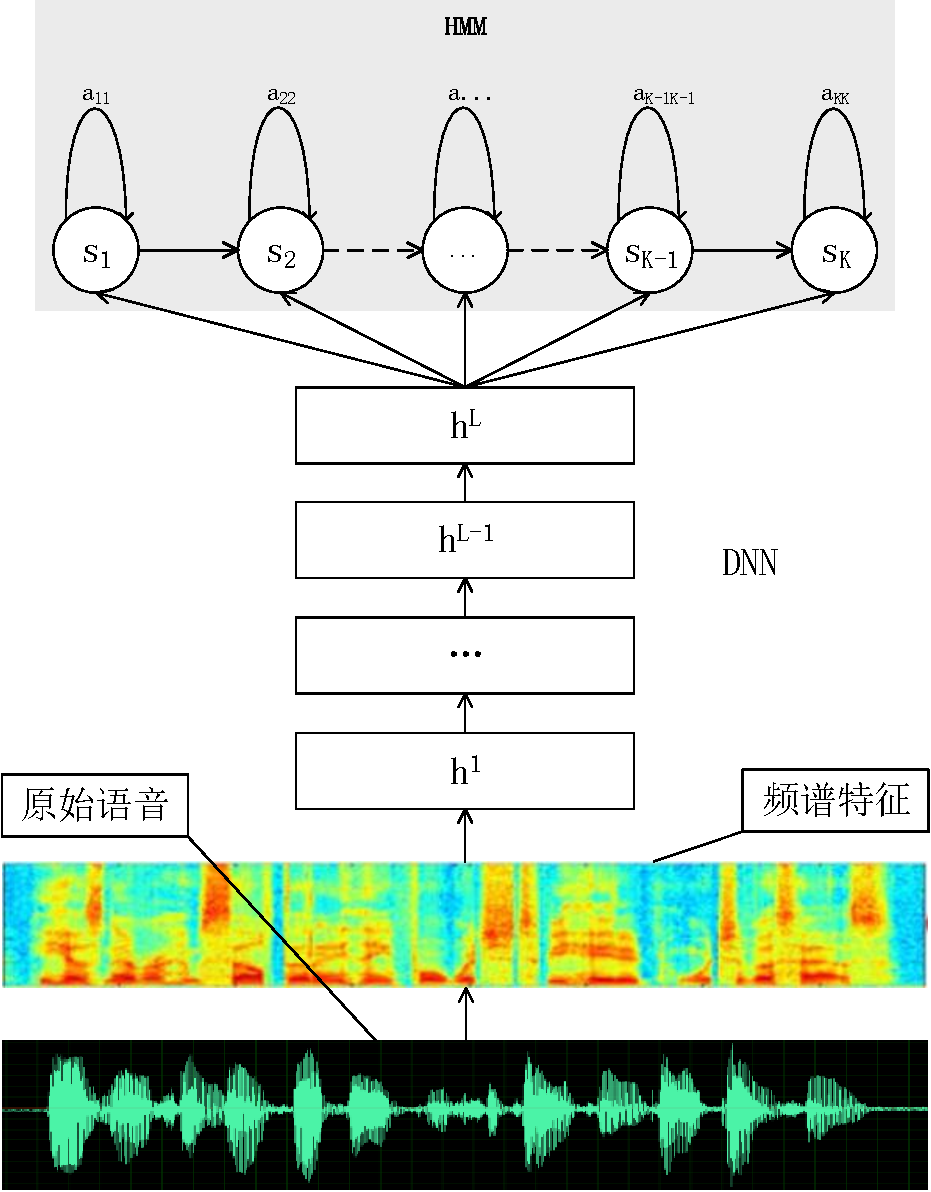
\includegraphics[width=0.6\textwidth]{figures/chapter3/hmmdnn-crop}
\caption{HMM-DL系统的基本原理}
\label{fig:hmmdnn}
\end{figure}


\section{全连接神经网络DNN}

深度神经网络DNN\ucite{bengio2012practical}(Deep Neural Network)是有多个(一般均大于2层)隐层的传统的多层感知机MLP(MultiLayer Perceptron)。
一个典型的神经网络由输入层;中间多个隐层和输出层组成。
如图\ref{fig:dnn}所示DNN,含有3个隐层,每个隐层有5个节点。
在一个$L+1$层的DNN中,我们定义输入层为第$0$层,输出层为第$L$层。

\begin{figure}
\centering
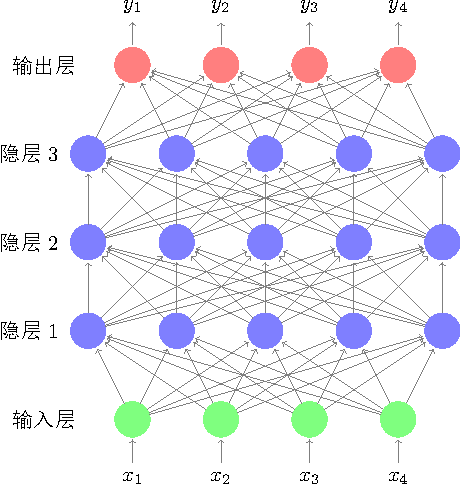
\includegraphics[width=0.5\textwidth]{figures/chapter3/dnn-crop}
\caption{DNN示例(该DNN由输入层、3个隐层和输出层组成)}
\label{fig:dnn}
\end{figure}

对于任意隐层$l$的任意节点$j$,有:
\[\begin{array}{l}
a_j^l = \sum\limits_{i = 1}^N {w_{ji}^l {x_i}^{l-1}+ b_j^l} \\
z_j^l = h(a_j^l)
\end{array}\]

其中,$i = 1,...,N$表示$l-1$层的节点数目,$a_j^l$表示第$l$层第$j$个节点的激励,
$a_j^l$经过激活函数$h(.)$作用得到$z_j^l$。
通常$h(.)$为非线性的、可导函数,
通过非线性函数增强神经网络的非线性映射能力,可导性则可以使神经网络通过梯度的方法行优化。

\subsection{激活函数}

在深度神经网络的实际应用中,最常用的激活函数是$sigmoid$函数:
\begin{equation}
s(z) = \frac{1}{{1 + {e^{ - z}}}}
\end{equation}
或者$tanh$函数:
\begin{equation}
\tanh (z) = \frac{{{e^z} - {e^{ - z}}}}{{{e^z} + {e^{ - z}}}}
\end{equation}
$sigmoid$函数将输入通过非线性函数映射到空间$(0,1)$;$tanh$函数的值域空间为$(-1,1)$,
其映射空间具有对称性。$ReLU$\ucite{glorot2011deep}是近年深度学习技术流行之后,又一个非常有效的激活函数:
\begin{equation} \label{equation:relu}
{\mathop{\rm Re}\nolimits} LU(z) = \max (0,z)
\end{equation}
$ReLU$激活函数预测具有稀疏性,这中预测特性提高了网络的泛化能力;另一方面,
如式\ref{equation:relu},$ReLU$的梯度形式简单,非0即1,有效的缓解了深度神经网络
训练中的梯度弥散问题;而且$ReLU$激活函数的计算更加简单,速度更快。
三种激活函数如图\ref{fig:activation}所示。

\begin{figure}
\centering
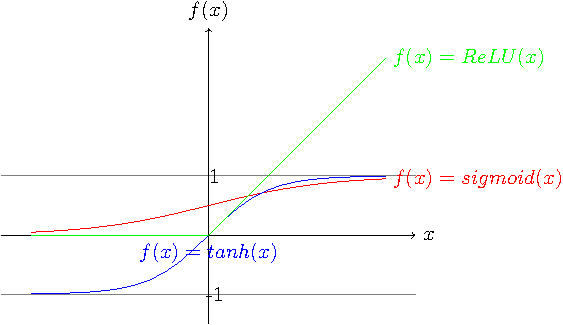
\includegraphics[width=0.6\textwidth]{figures/chapter3/activation-crop}
\caption{激活函数$sigmoid$,$tanh$,$ReLU$对比}
\label{fig:activation}
\end{figure}

激活函数的选择和深度神经网络密切相关,因此设计更好的激活函数也成为当下深度学习研究的热点之一,
最近的实验\ucite{zhang2014improving, zhang2015parameterised}表明,经过精心设计的激活函数能够
在一定程度上提高深度神经网络的性能。

\subsection{DNN训练}

DNN的训练即在损失函数确定后,使用误差方向传播BP(Back Propagation)算法计算参数梯度,
使用随机梯度下降SGD(Stochastic Gradient Descent)对模型中的参数进行更新。

一般来说,对于回归任务,使用最小均方误差MSE(Mean Suqare Error)损失函数:
\begin{equation}
E({\rm{w}}) = \frac{1}{2}\sum\limits_{n = 1}^N {\{ {y_n}}  - {t_n}{\} ^2}
\end{equation}
其中$y_n$为网络输出,$t_n$为标注,$N$为样本总数。

对于分类任务,首先应用softmax函数:
\begin{equation}
\label{equation:softmax}
{y_k} = \frac{{\exp ({a_k})}}{{\sum\limits_j {\exp ({a_{\rm{j}}})} }}
\end{equation}
计算在每个类别上的归一化后的概率,然后使用交叉熵CE(Cross Entropy)准则计算损失:
\begin{equation}
E(w) =  - \sum\limits_{n = 1}^N {\sum\limits_{k = 1}^K {{t_{kn}}\ln {y_k}} }
\end{equation}

根据\ref{section:hmmdl},基于深度神经网络的声学建模为典型的分类任务,
在输出层使用$softmax$函数做概率归一,使用交叉熵作为损失函数。

\section{卷积神经网络CNN}

CNN最早应用在图像领域,在基础DNN的结构上,CNN引进了局部滤波器,池化层和权值共享三个新思想。
深度学习在语音识别领域获得成功后,研究人员开始探索CNN在语音识别任务上的应用。

语音信号在频域上具有一定的局部特性,不同的音素在不同的局部频带上能量比较集中。
例如,非静音的音素在不同频带上有一定的共振峰。
在这些频带上应用局部滤波器或许能够提供对这些局部特征结构的更有效的表示,
这个特点是CNN能够应用在识别任务上的基础。

在语音识别中,CNN中使用卷积层能够对局部频域特征建模。
将输入语音信号分频带规整好之后,卷积层中每个卷积核的输入都为一定频段的语音信号。
假设输入信号$\textbf{x}$被分为$N$个频带$\textbf{x}= [\textbf{x}_1, \textbf{x}_2, ..., \textbf{x}_N]$,
其中向量$\textbf{x}_n$代表频段$n$。如图\ref{fig:cnn}所示,这个$\textbf{x}_n$可以包含原始频谱,一阶差分和二阶差分。
卷积层的激励被分为$K$个子带,每个频带包含$J$个滤波器的激励。
将每个子带的激励记作$\textbf{q}_k$ = $[q_{k,1}, q_{k,2}, ..., q_{k, J}]$,则有:
\begin{equation}
{{\rm{q}}_{k,j}} = h(\sum\limits_{n = 1}^{s - 1} {{\textbf{w}_{n,j}}\textbf{x}_{n{\rm{ + k}}}^T + {b_j})}
\end{equation}
其中,$h(.)$表示激活函数,$s$表示局部滤波器的宽度,$\textbf{w}_{n,j}$表示第$j$个滤波器的的第$n$维权重向量。


\begin{figure}
\centering
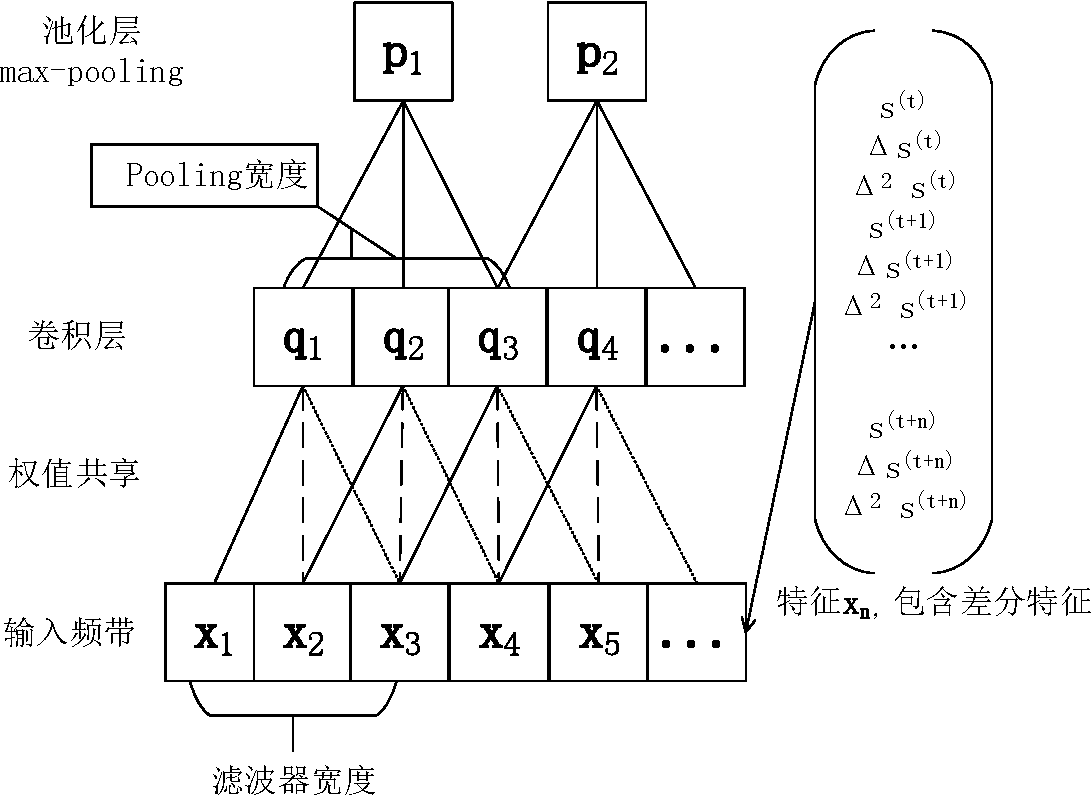
\includegraphics[width=0.6\textwidth]{figures/chapter3/cnn-crop}
\caption{CNN基本结构示意}
\label{fig:cnn}
\end{figure}

在CNN中,使用max-pooling(最大池化层)来保证局部不变性,max-pooling层一般位于卷积层之后,
作用在卷积层的激励输出上。max-pooling通过对局部激励取最大(max)操作,从而得到低分辨率的卷积层的输出,
这种表示更为抽象,更为鲁棒,随后作为高层神经网络的输入处理。
假设max-pooling操作共产生$M$个子带,将第$m$个子带的激励记作
$\textbf{p}_m$ = $[p_{m,1}, q_{m,2}, ..., q_{m, J}]$,则有:
\begin{equation}
{p_{m,j}} = \mathop {\max }\limits_{k = 1}^r ({q_{m \times n + k,j}})
\end{equation}
其中,$r$是pooling的大小,$n$是pooling的步长,一般小于$r$(这样允许临近的pooling操作可以有重叠),
图\ref{fig:cnn}中,pooling的大小为3,步长为2.

基于CNN的语音识别网络如图\ref{fig:cnnasr}所示。如上分析,CNN的输入为频域特征,
Fbank(Filter bank)特征是目前最为常用的频谱特征。
神经网络的底层为一层或者多层的CNN,用作频谱特征的抽取,之后会连接普通的DNN神经网络。
基于CNN的语音识别也是目前识别领域的研究热点之一,
一种趋势是直接CNN直接对原始音频Raw进行建模\ucite{palaz2015convolutional, sainath2016factored},
另一种趋势应用已经在图像上应用获得成功的Deep CNN\ucite{yu2016deep, xiong2016microsoft, sercu2016very, saon2015ibm}的结构到语音识别任务中。


\begin{figure}
\centering
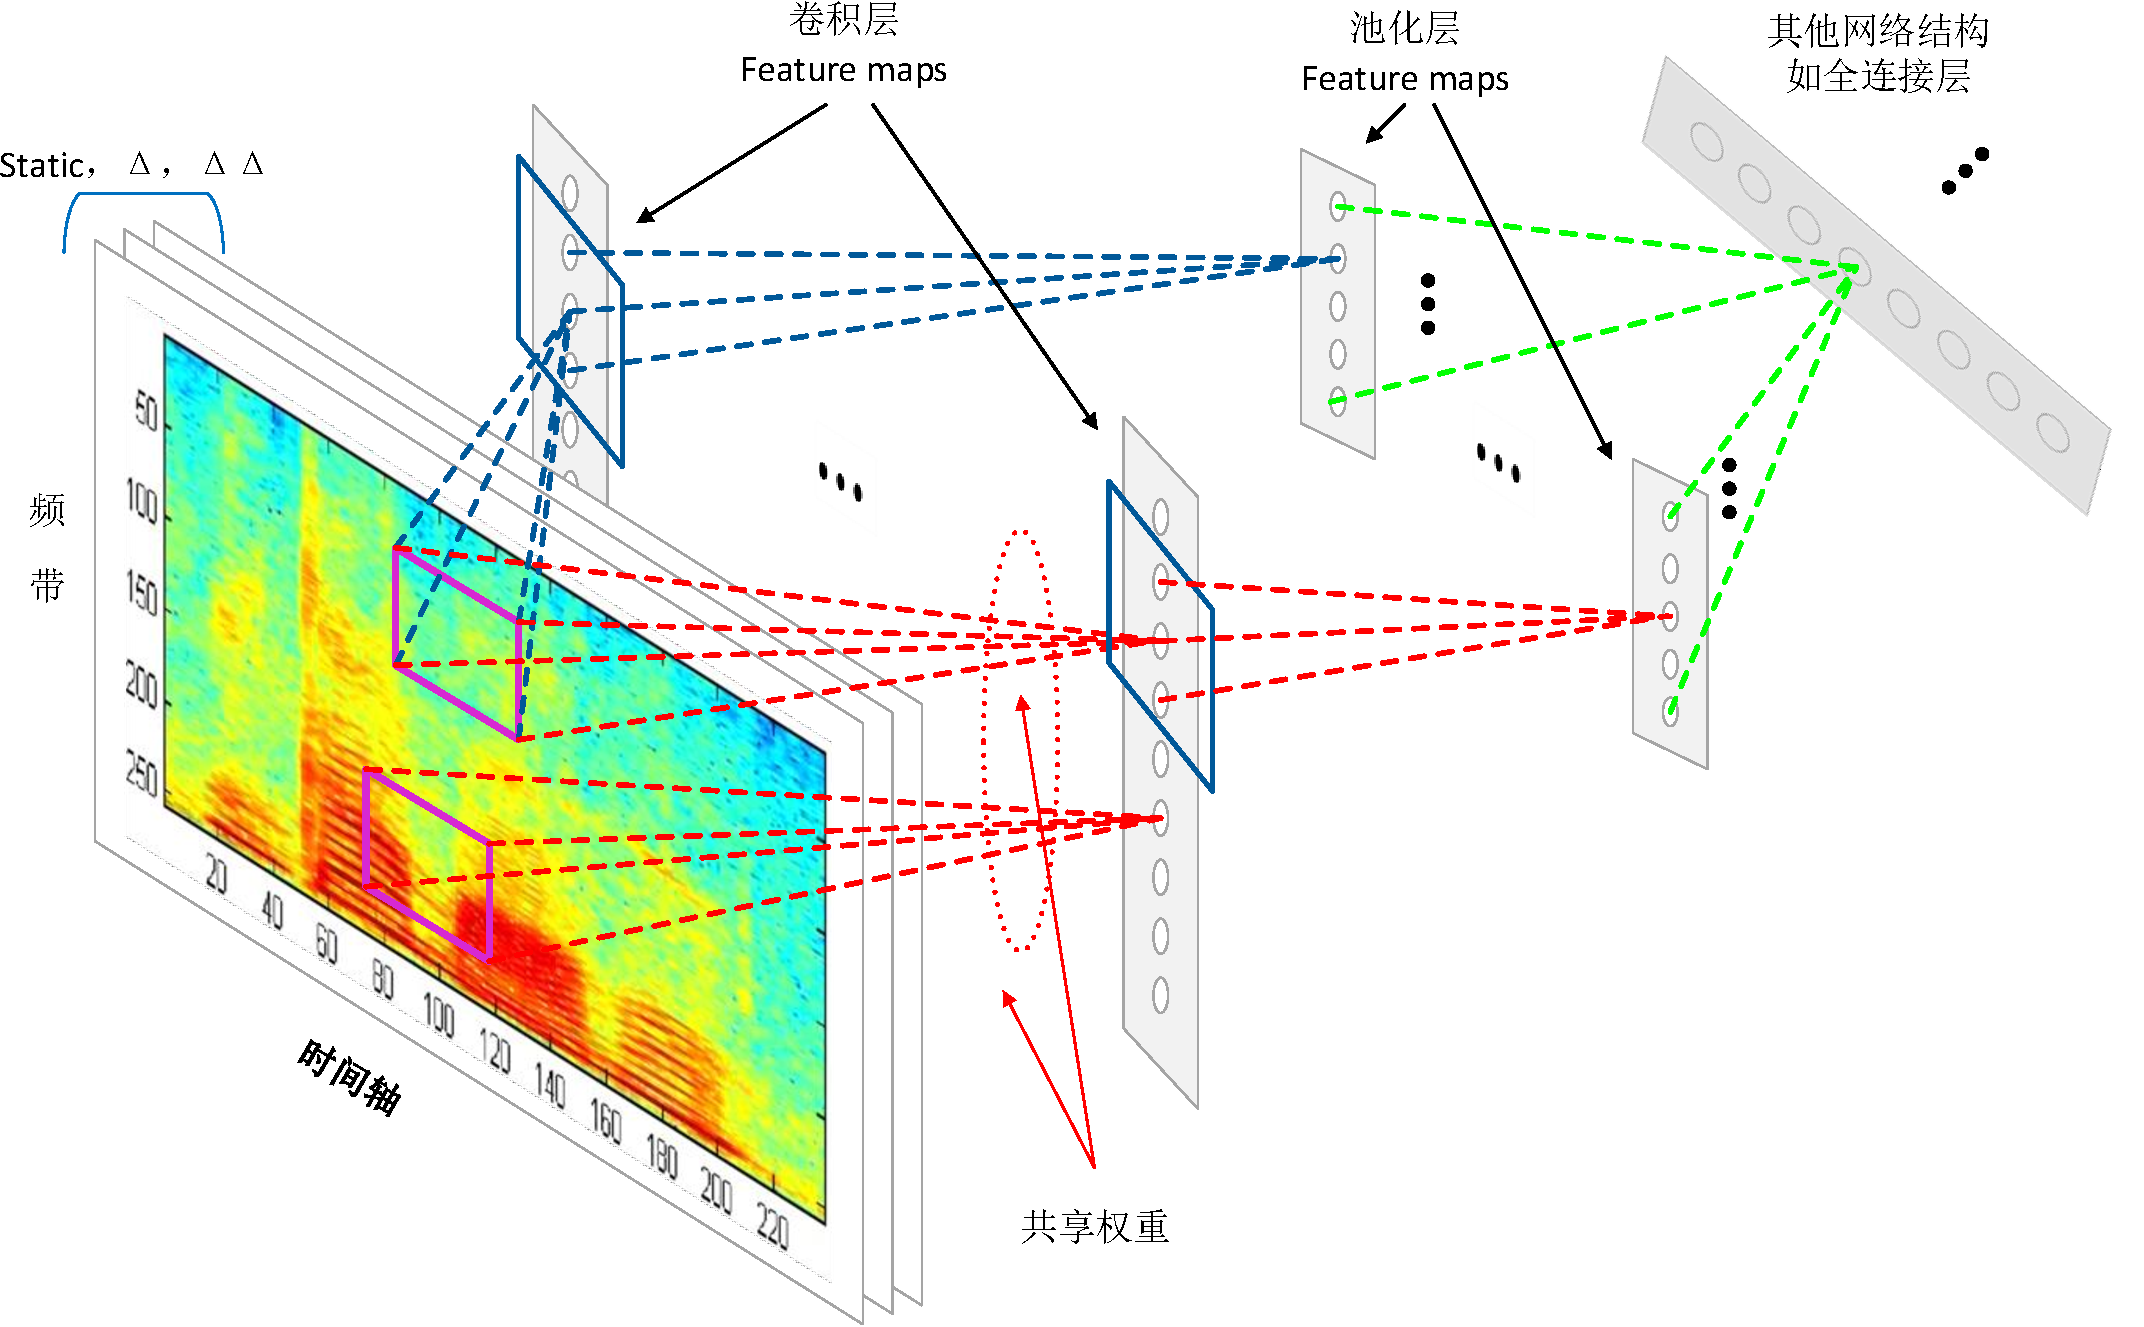
\includegraphics[width=0.8\textwidth]{figures/chapter3/cnnasr-crop}
\caption{基于CNN的声学模型}
\label{fig:cnnasr}
\end{figure}

\section{循环神经网络RNN}

循环神经网络RNN是一种带有Recurrent层的神经网络,循环Recurrent层中的神经元通过连接组成了一个有向环,
有向环使得循环神经网络有了内部状态和记忆单元的结构,从而赋予了循环神经网络记忆功能和对时序动态建模的能力。
如图\ref{fig:rnn}所示,循环神经网络RNN中循环层与全连接层的不同之处在于RNN的输出不仅是当前时刻下一层的输入,
同时还有上一时刻该循环层的输出,通过这样的结构,RNN能够在内部表示和学习序列中的历史信息。

RNN有许多变种的结构,这里我们介绍简单循环神经网络(记为RNN)和当前最为流行的长短时记忆(LSTM)的循环神经网络。


\begin{figure}
\centering
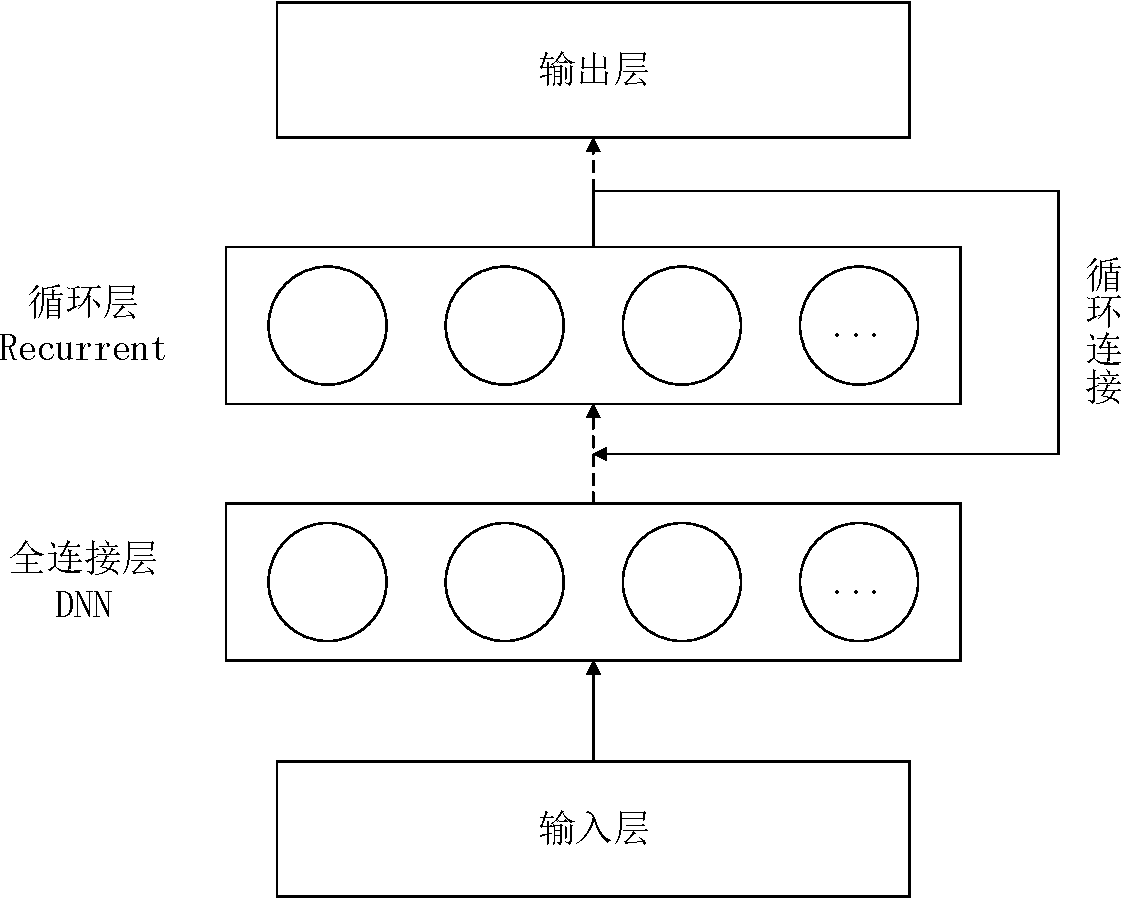
\includegraphics[width=0.5\textwidth]{figures/chapter3/rnn-crop}
\caption{循环神经网络RNN的基本结构}
\label{fig:rnn}
\end{figure}

\subsection{简单循环神经网络RNN}

简单循环神经网络RNN的结构和图\ref{fig:rnn}所示相同。
在任意时刻$t$,使用$\textbf{x}_t$表示前一层的$M$维输出,$\textbf{h}_t$是$N$维的隐状态向量,
则循环层RNN的输出可以表示为:
\begin{equation}
\textbf{h}_t = f({\textbf{W}_{xh}}{\textbf{x}_t} + {\textbf{W}_{hh}}{\textbf{h}_{t-1}})
\end{equation}
其中$f(.)$表示激活函数, $\textbf{W}_{xh}$是$N \times M$的连接前一层的权值矩阵,
$\textbf{W}_{hh}$是$N \times N$的连接$t-1$时刻该循环层输出$\textbf{h}_{t-1}$的权值矩阵,
$\textbf{h}_{t-1}$即是RNN的内部状态。

\subsection{LSTM}

RNN的结构相对简单,具有一定的对序列、时间轨迹建模能力,但在序列长度更大、问题更为复杂的任务中,
其建模能力则十分有限;此外,简单RNN的训练容易出现梯度爆炸或者弥散的问题,训练不够稳定。

为了解决上述问题,1997年,Hochreiter等人提出了LSTM\ucite{hochreiter1997long},
LSTM通过引入门结构复杂化RNN的基本结构,强化了建模能力;通过引入CEC(Constant Error Carousel)单元解决RNN训练中的不稳定问题。


LSTM的基本结构如图\ref{fig:lstm}左图所示,它的基本思想是利用不同类型的门来控制网络中的信息流。
LSTM结构中含有输入门、输出门、遗忘门三种基本门结构,门的基本输入为网络上一层的输出和该Recurrent层上一时刻的输出;
同时LSTM结构中引入cell单元,cell单元和隐层输出一起作用强化RNN的记忆功能。
LSTM的数据流向如下:
\begin{equation}
\begin{array}{l}
{{\rm{i}}_t} = \sigma ({W_{ix}}{x_t} + {W_{ih}}{h_{t - 1}}{\rm{ + }}{b_i})\\
{f_t} = \sigma ({W_{fx}}{x_t} + {W_{fh}}{h_{t - 1}}{\rm{ + }}{b_f})\\
{o_t} = \sigma ({W_{ox}}{x_t} + {W_{oh}}{h_{t - 1}}{\rm{ + }}{b_o})\\
{c_t} = {f_t} \odot {c_{t - 1}} + {i_t} \odot \tanh ({W_{cx}}{x_t} + {W_{ch}}{h_{t - 1}}{\rm{ + }}{b_c})\\
{h_t} = {o_t} \odot \tanh ({c_t})
\end{array}
\end{equation}
其中$i_t$表示输入门,$f_t$表示遗忘门,$o_t$表示输出门;$c_t$表示cell的内部值;
$\sigma$表示sigmoid激活函数;
$W$均为权值矩阵。

\begin{figure}
\centering
\subfigure[LSTM]{
\begin{minipage}[b]{0.4\textwidth}
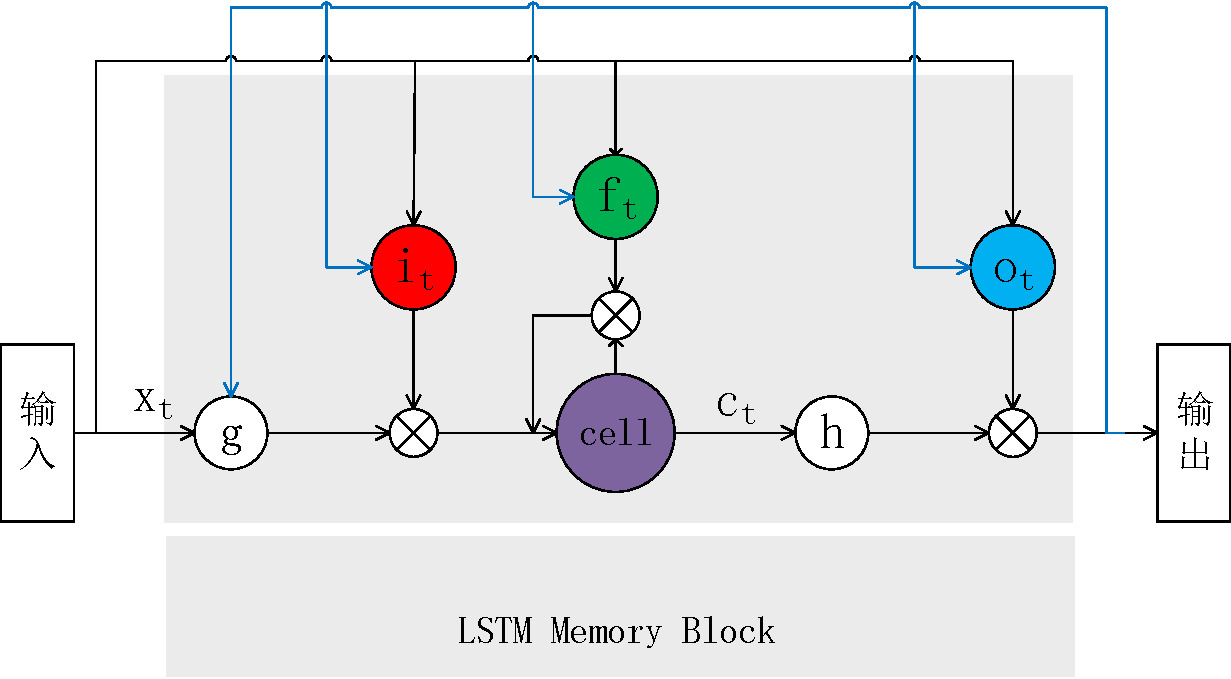
\includegraphics[width=1\textwidth]{figures/chapter3/lstm-crop}
\end{minipage}
}
\subfigure[LSTMP]{
\begin{minipage}[b]{0.45\textwidth}
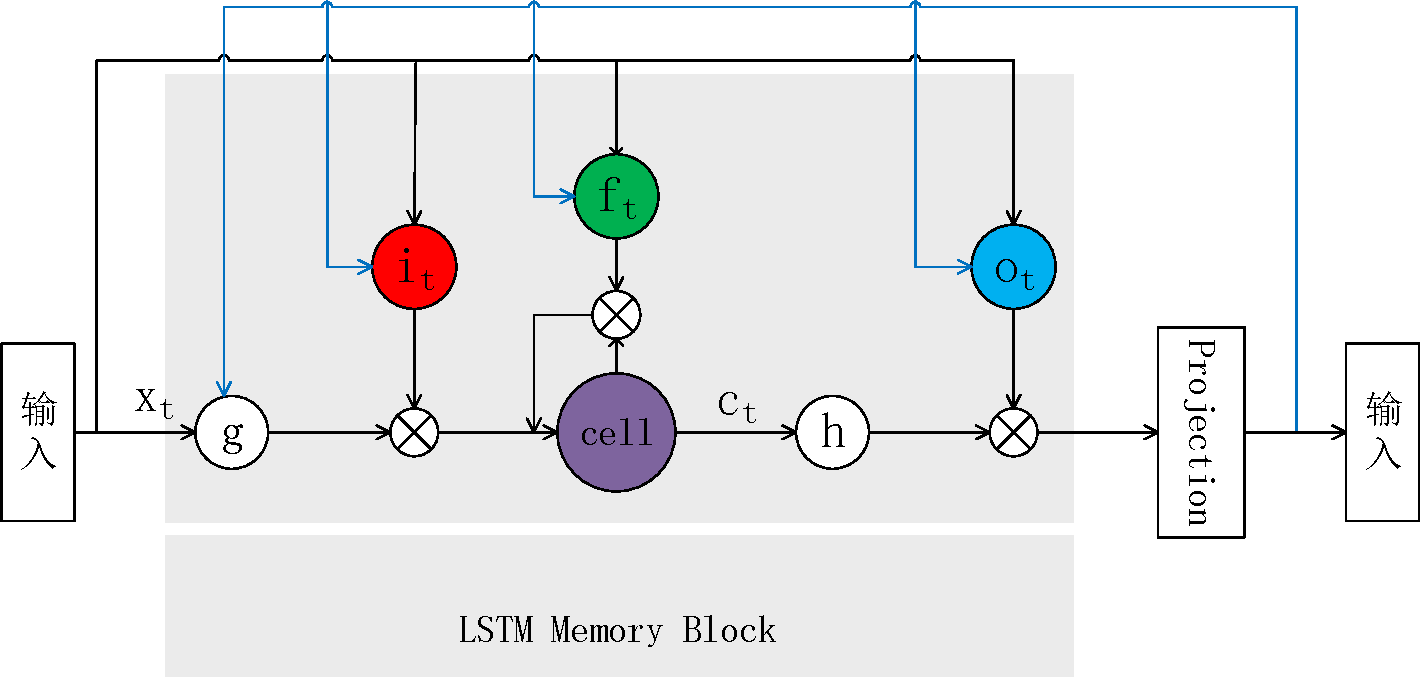
\includegraphics[width=1\textwidth]{figures/chapter3/lstmp-crop}
\end{minipage}
}
 \caption{LSTM的基本结构示意} \label{fig:lstm}
\end{figure}

标准的LSTM中,循环的连接直接从Memory Block的输出连接至Memory Block的输入和各个控制门。
2014年,Google首次将LSTM应用于大词汇量连续语音识别\ucite{sak2014long, sak2014long_lvsr},
Google研究人员将标准LSTM的输出连接到一个Projection层,然后将Projection的输出作为循环连接
到Memory Block的输入和控制门,这种结构成为LSTMP(LSTM with Projection),如图\ref{fig:lstm}
右图所示。在一般的设置中,LSTMP中的Projection层的节点数小于LSTMP中Memory Block的个数(比如Memory Block数量为1024,Projection可设为512),
这样有效减小了循环连接矩阵的大小。
通过Projection层,一方面减小了网络的参数数量,另一方面这种改进在声学模型上比标准LSTM取得更好的效果。
LSTMP的数据流向如下:
\begin{equation}
\label{equation:lstmp}
\begin{array}{l}
{{\rm{i}}_t} = \sigma ({W_{ix}}{x_t} + {W_{ih}}{h_{t - 1}}{\rm{ + }}{b_i})\\
{f_t} = \sigma ({W_{fx}}{x_t} + {W_{fh}}{h_{t - 1}}{\rm{ + }}{b_f})\\
{o_t} = \sigma ({W_{ox}}{x_t} + {W_{oh}}{h_{t - 1}}{\rm{ + }}{b_o})\\
{c_t} = {f_t} \odot {c_{t - 1}} + {i_t} \odot \tanh ({W_{cx}}{x_t} + {W_{ch}}{h_{t - 1}}{\rm{ + }}{b_c})\\
{{\rm{m}}_t} = {o_t} \odot \tanh ({c_t})\\
{h_t} = {W_m}{m_t}
\end{array}
\end{equation}
其中,$W_m$为Projection层的变换矩阵。由式\ref{equation:lstmp}可以看出,在LSTMP中Memory Block的输出$m_t$并不直接回连到自身,
而是先通过Projection层的$W_m$做矩阵变化后,再回连到Memory Block。

\section{混合神经网络CLDNN}

目前,在大多数语音识别任务上,基于CNN和LSTM的声学模型均能取得比基于DNN的声学模型更好的效果。
那么一个很自然的想法就是,能否将三者结合使用,各取所长,相互补充。
CNN对频率各种变化具有较好的不变性,长于提取局部特性和特征;
LSTM有记忆功能,长于对时序序列建模;
DNN长于特征抽象和映射。
2015年,Google的工作\ucite{sainath2015convolutional}表明,通过三种网络结合的混合结构CLDNN(CNN,LSTM,DNN),
在大词汇量连续语音识别任务上,均能比LSTM取得4$\sim$6\%的收益。

\subsection{CLDNN的基本结构}

Google提出的CLDNN的基本结构如图\ref{fig:cldnn}左图所示,
首先,为了对频率变化更好的建模,在网络底层使用1层或多层的卷积层CNN,使用卷积和池化操作;
网络中间是多层的LSTM结构,对CNN的输出进行时序建模;
LSTM层之后紧接多层的DNN,用于深化网络结构,提供更强大的建模能力。


\begin{figure}
\centering
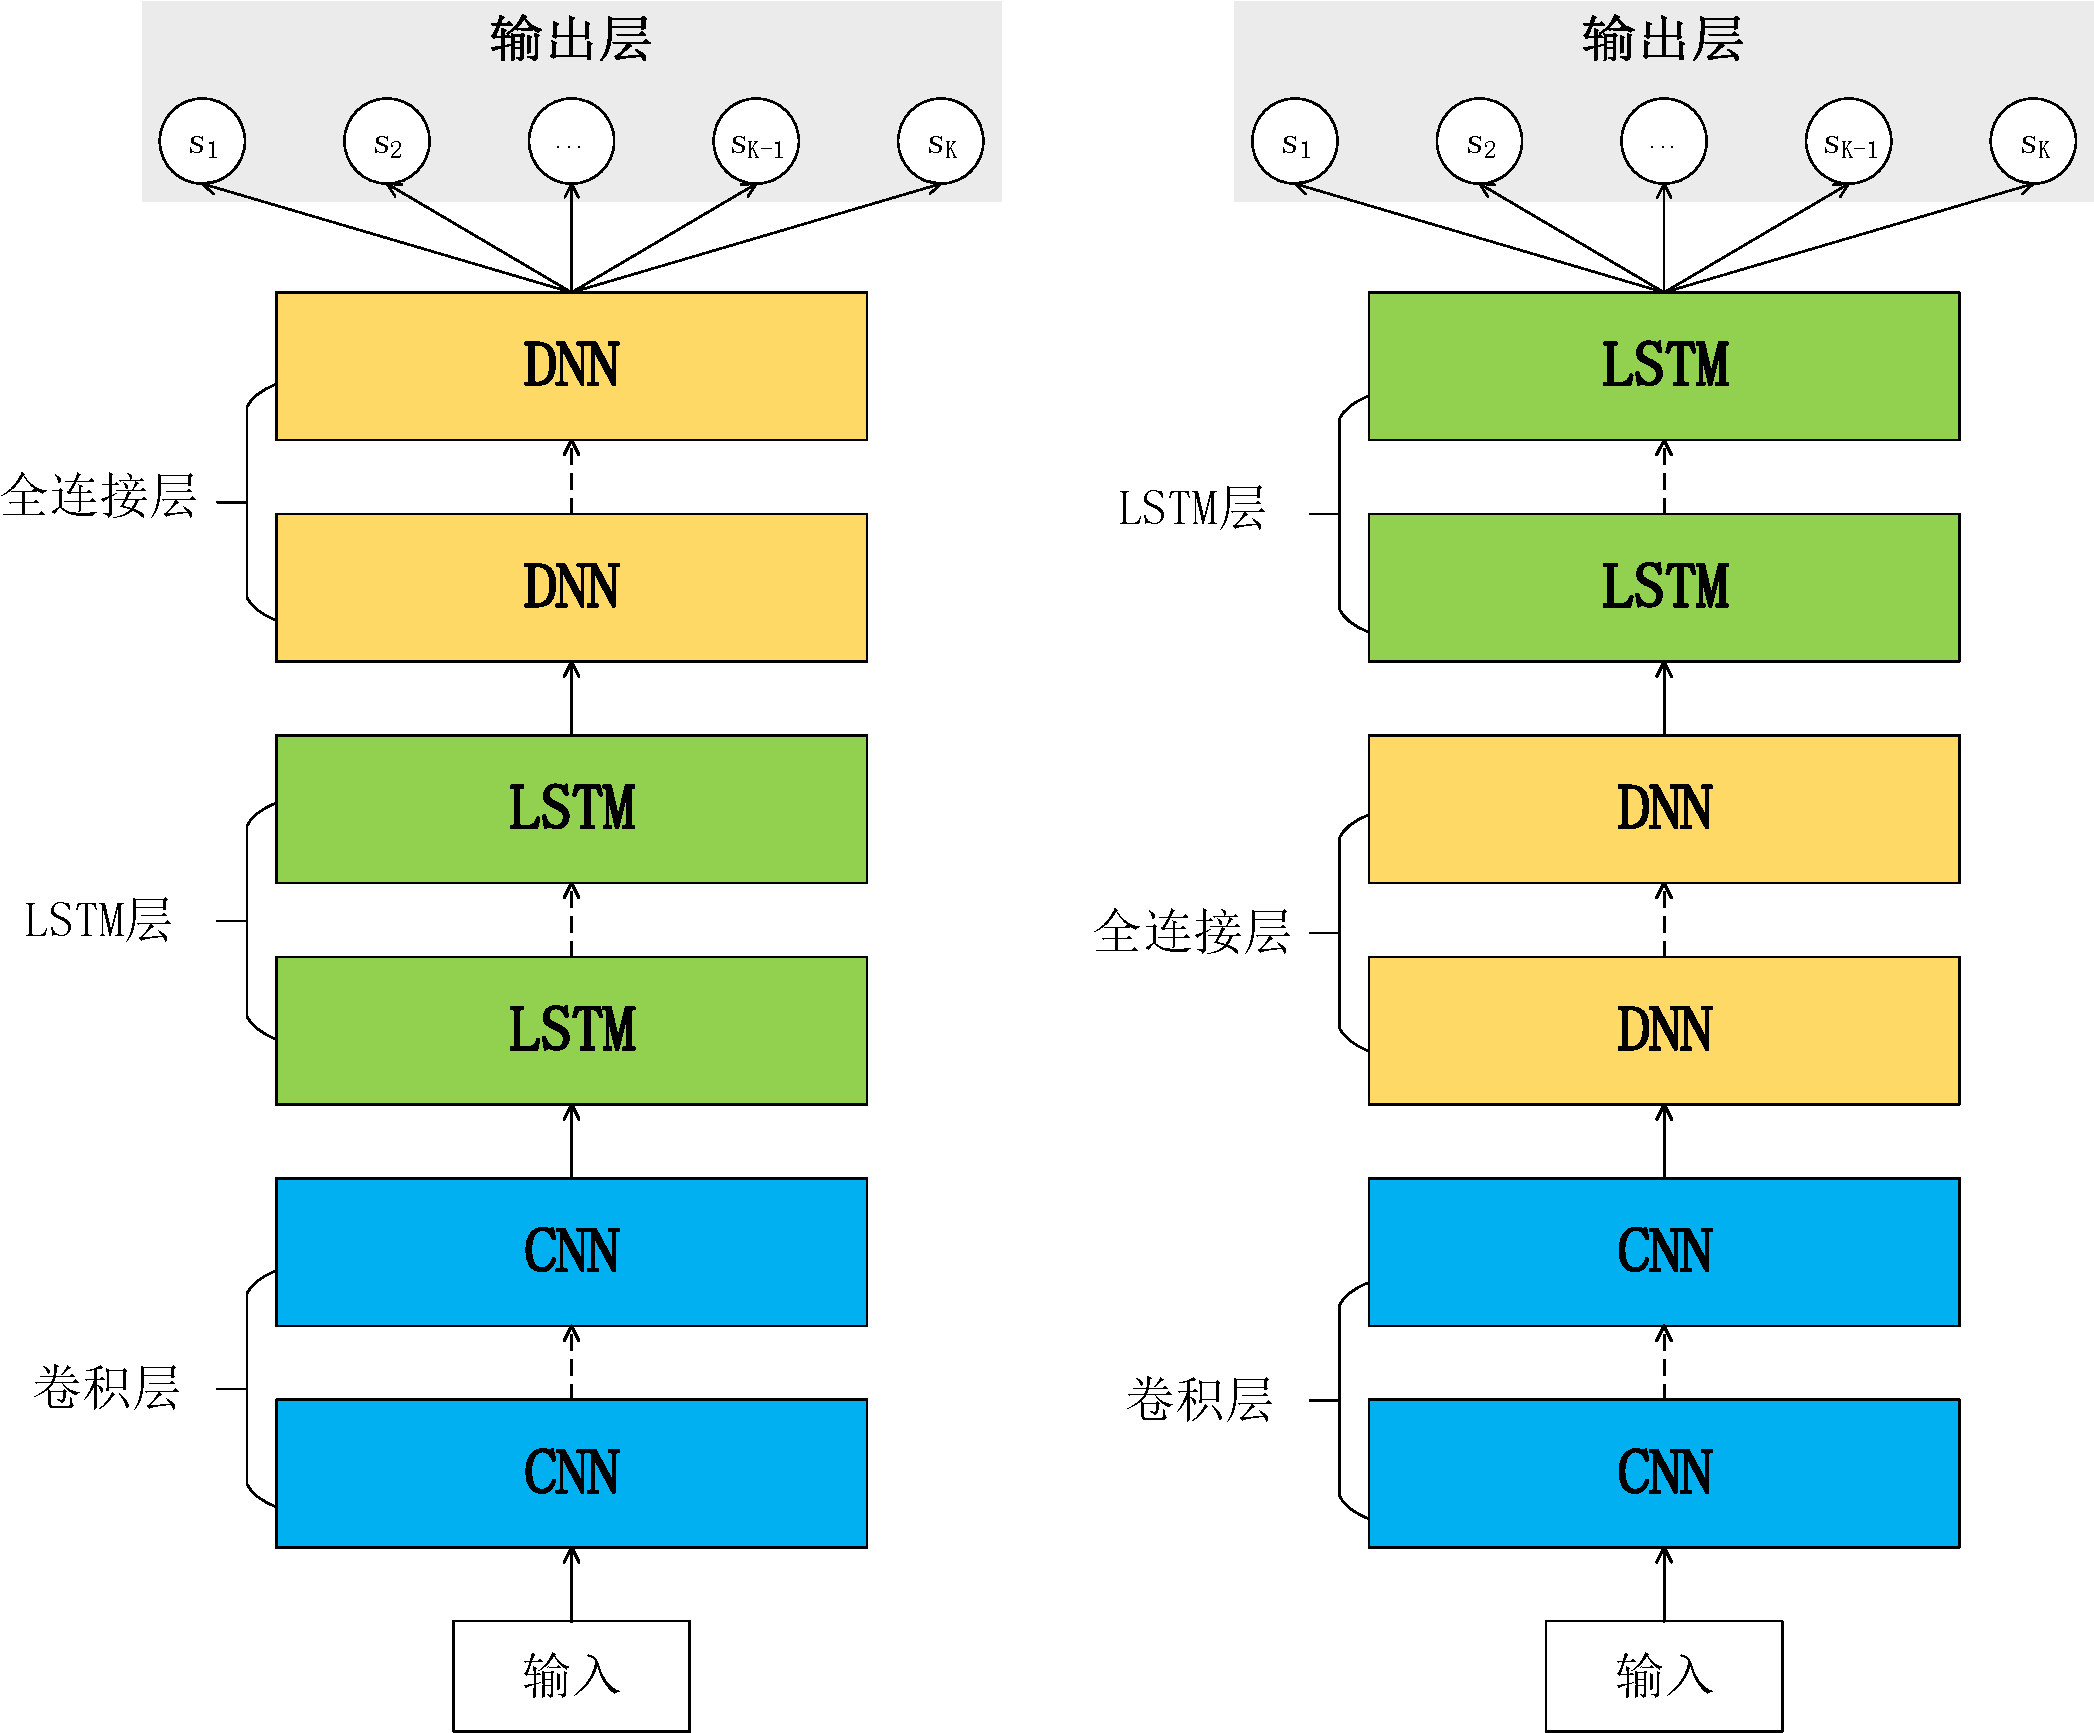
\includegraphics[width=0.8\textwidth]{figures/chapter3/cldnn-crop}
\caption{CLDNN的基本结构}
\label{fig:cldnn}
\end{figure}

在实际的应用过程中,我们发现可以做一些顺序上的调整。
声学模型的输入是频谱特征,所以长于频谱建模的CNN必须置于网络最下层。
DNN和LSTM层的位置是可调的,LSTM层也可以放在CNN和DNN之后,如图\ref{fig:cldnn}右图所示,
目前证明两种结构均能取得不错的效果。LSTM层放在CNN之后一个潜在的优点是相对DNN,
LSTM的梯度更不稳定,根据误差反向传播原理,深度神经网络梯度传递到低层时容易出现梯度爆炸或弥散的问题,
LSTM位置越靠近顶层,反馈回来的梯度稳定性能更好一点,从而整个网络的稳定性更好;
另一个潜在的优点是,基于已有DNN和CNN的识别网络(相当于已经预训练好的深层结构),
可以直接在其输出层之前插入多层的LSTM,快速得到CLDNN的结构训练并部署,
并与之前的系统进行比较。


\subsection{CLDNN跳帧训练}

DNN在通用语音识别上的取得成功后,人们迫切的希望能够将基于DNN的声学模型应用于手机等的嵌入式设备。
但DNN计算量庞大,在这些设备上往往是性能瓶颈,在实际应用时如何减小和优化DNN的计算量成为硬需。
跳帧训练最早在基于DNN\ucite{vanhoucke2013multiframe}的语音识别任务中提出,
当时在保证性能基本不下降的情况下,有效的成倍的减小了计算量。

CNN、LSTM和CLDNN应用成功,使跳帧训练的应用更为广泛。
CNN的输入基于频谱特征,在输入层上需要依赖当前帧的左右上下文(Context),即需要特征拼帧输入,
这样在1帧的输入中,其实已经包含了左右几帧的特征信息。
LSTM的强大的序列建模能力,比DNN能够更好的进行跳帧时的平滑预测;
CLDNN结合了两者的优点,跳帧预测能力则更强。
一般语音训练的语料平均长度在4到6秒,语音识别特征以10ms为帧移,所以特征的帧率为100帧/秒,
且通过拼帧后,相邻帧之间还会有特征重叠。
近来的研究\ucite{sak2015fast, amodei2015deep, miao2016simplifying}表明,这样的高帧率和重叠实际上是有冗余的。

\begin{figure}
\centering
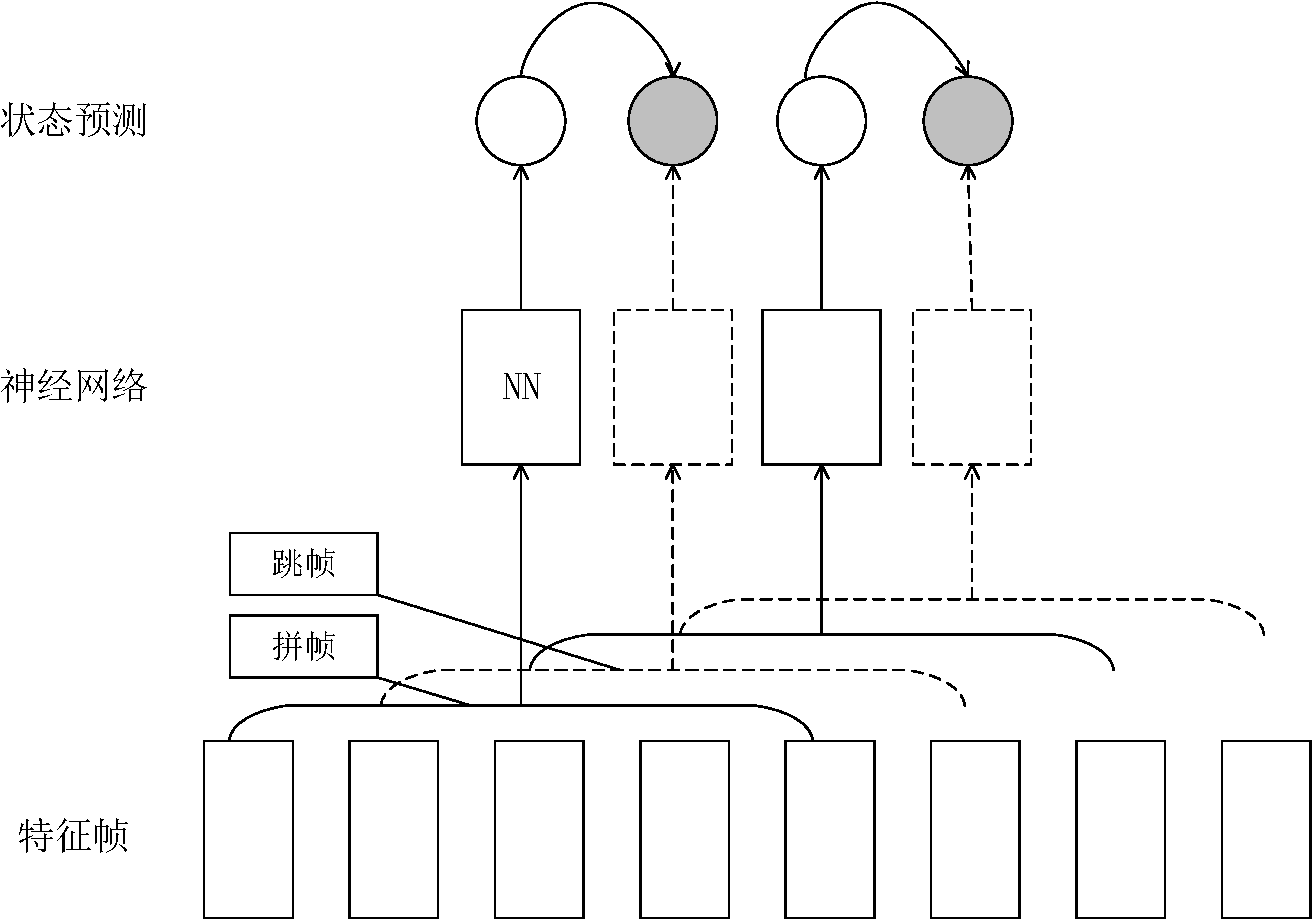
\includegraphics[width=0.5\textwidth]{figures/chapter3/skip-crop}
\caption{跳帧训练(跳1帧,虚线表示被跳过的训练数据)}
\label{fig:skip}
\end{figure}


跳帧训练的基本结构如图\ref{fig:skip}所示,网络输入层通过拼帧形成宽上下文,图中共拼5帧,每2帧跳1帧,
图中虚线表示被跳过的训练数据。跳帧训练时忽略被跳过的训练数据,所以能够有效成倍减小训练序列长度,
相当于对拼帧后的训练数据进行了降采样。
在识别预测时,有两种方法。
第一,仅使用选中帧(图中实线)进行预测,被跳过状态(图中灰色圈)的预测直接拷贝前一个选中帧的神经网络预测,称之为Copy模式;
第二,假设跳帧训练设置为N帧跳1帧,则将预测序列按按顺序分为N份$\{0, N, 2N, ...\}$, $\{1, N+1, 2N+1, ...\}$, ..., $\{N-1, 2N-1, 3N-1, ...\}$,
分别在网络中进行前向打分,最后将N份预测按顺序组织起来作为整体的预测,即$\{0, 1, ..., N, ..., 2N, ...\}$,称之为Split模式。


跳帧训练能有效的减小序列长度,提高训练速度,并加倍减少识别时神经网络的计算量。
在CTC的训练任务中,通过跳帧训练减小输入序列的长度,能有效提高CTC的训练的稳定性。

\section{Batch Normalization}

一般在准备深度神经网络的训练数据时,需要对训练数据进行归一化预处理。
最常用的的归一化操作使均值方差归一化MVN(Mean Variance Normalization),
即将训练数据通过减均值除以标准差的操作归一化到标准的正态分布。
通过归一化MVN操作,将输入映射到标准的高斯空间,利于训练的收敛性和模型效果。

2015年,Google的工作\ucite{ioffe2015batch}表明,同样可以在神经网络的中间层的输入上进行类似的MVN操作。
训练深度神经网络是个复杂多变的过程,神经网络中每一层的输入的分布都会随着训练逐渐改变,
这导致了神经网络的收敛速度慢,并且需要设置较小的学习率和更精细的初始化来保证神经网络的收敛性。
所以,类似输入层的归一化,可以通过归一化网络每一层的输入来解决该问题。

在训练中,对每一层的输入进行归一化时,由于计算全局的归一化代价很高,并且不可导,即不能使用梯度方法进行优化。
神经网络在训练过程中,使用mini-batch训练方法,mini-batch中含有多个训练样本。
所以,在归一化时,对归一化进行如下简化:
\begin{enumerate}
\item 使用mini-batch的归一化,即使用mini-batch的均值和方差替代全局的均值和方差。
\item 假设各维输入独立不相关,对每一层输入的每一维进行独立的归一化。
\end{enumerate}

假设mini-batch~${\rm B}$的大小为N,假设$x_k$表示${\rm B}$中任意一维输入的第$k$个样本,即
\begin{equation}
{\rm B}{\rm{ = }}\{ {x_1},{x_2},...,{x_N}\}
\end{equation}
计算每一维的均值和方差:
\begin{equation}
\begin{array}{l}
{\mu _{\rm B}} = \frac{1}{N}\sum\limits_{i = 1}^N {{x_i}} \\
\sigma _{\rm B}^2 = \frac{1}{N}\sum\limits_{i = 1}^N {({x_i} - } {\mu _{\rm B}}{)^2}
\end{array}
\end{equation}
则归一化的输出${\hat x}_i$可以表示为:
\begin{equation}
{{\hat x}_i} = \frac{{{x_i} - {\mu _{\rm B}}}}{{\sqrt {\sigma _{\rm B}^2 + \varepsilon } }}
\end{equation}
其中,$\varepsilon$是为防止除0引入的常量加项。

注意到仅仅使用这种简单的归一化可能会改变神经网络层的表征能力。
例如,tanh的输入通过这种简单归一化后,其激励会集中在坐标轴附近,
如图\ref{fig:activation},在坐标轴附近,tanh函数为近似的线性函数,
所以简单归一化必然降低了tanh的非线性映射能力。
为了解决该问题,使得变化满足镜像变换的能力,即从自身映射到自身,
对于每一维输入$x_i$引入一对参数$\gamma _i$和$\beta _i$,并且:
\begin{equation}
{y_i}{\rm{ = }}{\gamma _i}{{\hat x}_i} + {\beta _i}
\end{equation}
$y_i$是最终Batch Normalization的输出,当
${\gamma _i} = \sqrt {\sigma _{\rm B}^2 + \varepsilon }$
并且${\beta _i} = {\mu _{\rm B}}$时:
\begin{equation}
{y_i} = {x_i}
\end{equation}
即实现了镜像变换。$\gamma _i$和$\beta _i$是可以训练的参数,并且可导,
可以通过神经网络的优化同步训练。

在训练过程中,可以统计所有训练数据在神经网络每一层输入做前向时产生的均值和方差。
因此,在测试时,可以直接使用由训练数据统计的均值和方差。
假设训练过程中统计的任意一维输入$x_i$的全局均值为$E\left[ {{x_i}} \right]$,
全局方差为$Var[{x_i}]$,则在预测时:
\begin{equation}
\begin{array}{l}
{{\hat x}_i} = \frac{{{x_i} - E\left[ {{x_i}} \right]}}{{\sqrt {Var[{x_i}] + \varepsilon } }}\\
{y_i}{\rm{ = }}{\gamma _i}{{\hat x}_i} + {\beta _i}
\end{array}
\end{equation}

在深度神经网络中,对于普通的全连接层,Batch Normalization的位置在线性变换之后,激活函数之前,即:
\begin{equation}
y = f(BN(Wx + b))
\end{equation}
在卷积神经网络CNN中,对卷积后的每维输出均进行归一化,所以Batch Normalization的位置在卷积层和Max Pooling层
之间。对于LSTM,研究\ucite{laurent2015batch}表明,在多个位置做归一化并不有效,而仅对输入做Batch Normalization
证明有效。

众多的实验\ucite{ioffe2015batch, laurent2015batch, amodei2015deep, }表明,使用Batch Normalization不仅可以设置更大的学习率,而且可以加快网络的收敛速度,
并进一步提高模型的效果。因此,在神经网络的训练过程中如若遇到收敛速度慢或者梯度问题导致无法
收敛时,可以尝试使用Batch Normalizaiton来解决。目前,Batch Normalization已作为深度神经网络
优化的标配之一。

\section{实验} 